\chapter{Implementacja}

Implementacja projektu została zrealizowana przy użyciu kilku kluczowych technologii i narzędzi wspierających proces uczenia modelu oraz monitorowanie eksperymentów. Poniżej przedstawiono najważniejsze szczegóły implementacyjne oraz architekturę systemu.

\section{Technologie}

\begin{itemize}
	\item \textbf{PyTorch:} Biblioteka do budowy i trenowania modelu DQN (Deep Q-Network) oraz implementacji warstw konwolucyjnych, w pełni połączonych i mechanizmów propagacji gradientów.
	\item \textbf{Weights and Biases (WandB):} Narzędzie do monitorowania eksperymentów, umożliwiające śledzenie hiperparametrów, wyników oraz wizualizację metryk uczenia.
	\item \textbf{Własny algorytm DQN:} Algorytm Double Q-Learning został zaimplementowany ręcznie w celu lepszego dostosowania do specyficznych wymagań projektu.
\end{itemize}
\section{Architektura systemu}

Cały system został zaprojektowany do pracy na zdalnej maszynie wyposażonej w GPU NVIDIA, gdzie jednocześnie działa wiele procesów związanych z różnymi modelami. System korzysta z dodatkowych narzędzi, takich jak \texttt{WandB} do monitorowania i archiwizacji oraz \texttt{SQLite} do przechowywania parametrów modelu i stanu optymalizatora. Architektura systemu jest przedstawiona na rysunku~\ref{fig:system_architecture}.

\begin{figure}[h!]
	\resizebox{\textwidth}{!}{
		\centering
		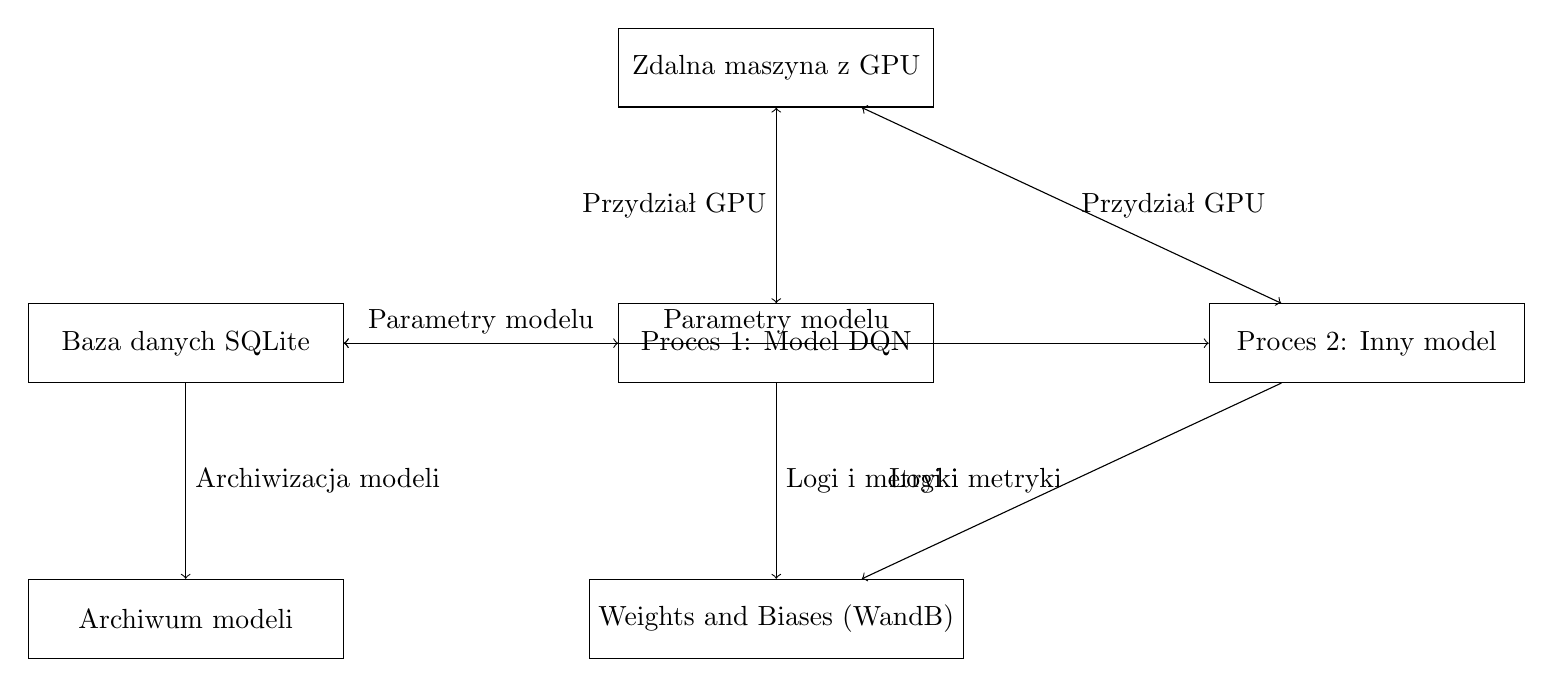
\begin{tikzpicture}[node distance=2.5cm]
			% Nodes
			\node[draw, rectangle, minimum width=4cm, minimum height=1cm] (gpu) {Zdalna maszyna z GPU};
			\node[draw, rectangle, minimum width=4cm, minimum height=1cm, below of=gpu, yshift=-1cm] (process1) {Proces 1: Model DQN};
			\node[draw, rectangle, minimum width=4cm, minimum height=1cm, right of=process1, xshift=5cm] (process2) {Proces 2: Inny model};
			\node[draw, rectangle, minimum width=4cm, minimum height=1cm, left of=process1, xshift=-5cm] (sqlite) {Baza danych SQLite};
			\node[draw, rectangle, minimum width=4cm, minimum height=1cm, below of=process1, yshift=-1cm] (wandb) {Weights and Biases (WandB)};
			\node[draw, rectangle, minimum width=4cm, minimum height=1cm, below of=sqlite, yshift=-1cm] (archive) {Archiwum modeli};

			% Arrows
			\draw[<->] (gpu) -- (process1) node[midway, left] {Przydział GPU};
			\draw[<->] (gpu) -- (process2) node[midway, right] {Przydział GPU};
			\draw[<->] (process1) -- (sqlite) node[midway, above] {Parametry modelu};
			\draw[<->] (process2) -- (sqlite) node[midway, above] {Parametry modelu};
			\draw[->] (process1) -- (wandb) node[midway, right] {Logi i metryki};
			\draw[->] (process2) -- (wandb) node[midway, left] {Logi i metryki};
			\draw[->] (sqlite) -- (archive) node[midway, right] {Archiwizacja modeli};
		\end{tikzpicture}
	}
	\caption{Architektura systemu implementacji}
	\label{fig:system_architecture}
\end{figure}

\section{Szczegóły implementacyjne}

\begin{itemize}
	\item \textbf{Zdalna maszyna z GPU:} System działa na serwerze wyposażonym w GPU NVIDIA, umożliwiając równoczesne trenowanie kilku modeli. GPU przydzielane są do poszczególnych procesów w zależności od obciążenia.
	\item \textbf{Weights and Biases (WandB):} WandB jest używane do monitorowania eksperymentów. Zapisuje logi, metryki (np. stratę i nagrody) oraz regularnie archiwizuje stany modelu i optymalizatora.
	\item \textbf{SQLite:} Lekka baza danych SQLite przechowuje parametry modelu, stany optymalizatora oraz inne dane konfiguracyjne, co umożliwia łatwe wznowienie treningu lub analizę po zakończeniu procesu.
	\item \textbf{Archiwum modeli:} Modele i stany optymalizatora są regularnie zapisywane w formacie binarnym w lokalnym archiwum, co pozwala na późniejsze wykorzystanie i ewaluację.
	\item \textbf{Procesy równoległe:} Na maszynie uruchamiane są równocześnie różne procesy, z których każdy zajmuje się trenowaniem innego modelu. WandB synchronizuje dane z każdego procesu w czasie rzeczywistym.
\end{itemize}

\section{Monitorowanie i archiwizacja}

Dzięki integracji z WandB i SQLite proces treningu jest w pełni monitorowany. WandB umożliwia wizualizację wyników w czasie rzeczywistym, a SQLite zapewnia
\section{Uruchomienie systemu}

System działa na zdalnej maszynie, co wymaga:
\begin{itemize}
	\item Konfiguracji środowiska wirtualnego z bibliotekami \texttt{PyTorch}, \texttt{WandB} oraz dodatkowymi zależnościami.
	\item Połączenia z serwerem WandB w celu monitorowania eksperymentów.
	\item Uruchomienia emulatora NES i algorytmu DQN na zdalnej maszynie wyposażonej w GPU.
\end{itemize}

Proces treningu obejmuje iteracyjne aktualizowanie modelu DQN, przesyłanie wyników do WandB oraz przechowywanie danych w Replay Buffer w celu stabilizacji procesu uczenia.
